\section{Methodology}


Our proposed framework, AnalogSAGE, translates analog circuit specifications into executable designs through an iterative, memory-augmented reasoning process. As illustrated in Figure~\ref{fig:methodology_overview}, this process is driven by three sequential agents: a \emph{Topology Selection Agent} proposes an initial architecture, a \emph{Topology Refinement Agent} modifies its structure to resolve design issues, and a \emph{Parameter Optimization Agent} determines the final numerical values for each device.


Crucially, the reasoning of the agents is supported by four \textit{Stratified Memory Layers}, which form the cognitive backbone of the system. \textit{Evolution Memory} transfers high-level insights across different design tasks, while \textit{Introspective Optimization} enables self-correction by learning from prior iterations within the same task. \textit{Stage Context Fusion} maintains a compressed summary of the current design state, and \textit{Analog Design Experience} grounds the agents with verified domain knowledge.

This tight integration of agents and memory allows \textit{AnalogSAGE} to operate as a self-evolving system, continually improving its design capabilities across both iterations and tasks. Here, a design task is defined by a set of specifications that is considered a pass only when all requirements are satisfied after simulation. Because initial solutions may fail, multiple design iterations are often required within a single task to refine the solution until the specifications are met, or the design still fails after reaching the maximum number of iterations.



\subsection{Stage agents}




The design process is divided into three reasoning stages, each controlled by a stage agent. Agents operate with different objectives: selecting a topology, refining its structure, and determining numerical parameter values. All agents share the same memory layer organization, but receive different tool feedback and contextual information. Information flows forward across stages, while compressed feedback is passed backward through the memory system, forming a closed loop that can iteratively solve the design task.


\subsubsection{Topology Selection Agent}




The \emph{Topology Selection Agent} initiates the design process by translating textual performance specifications into a concrete circuit architecture in netlist format. To avoid generating invalid topologies, the agent first queries the \emph{Stratified Memory Layers} for contextual signals derived from past design tasks and previous iterations. Conditioned on this context, it formulates a natural language description of the target architecture. This description is passed to the \emph{Candidates Module}, which retrieves the best-matching validated topology from the database. This retrieval-based initialization ensures that the design process begins from a structurally sound foundation.


\subsubsection{Topology Refinement Agent}


Once a promising topology is identified, the design flow enters an iterative refinement stage. Based on the gathered context, the agent performs localized structural modifications, such as adjusting bias networks or compensation paths. The refined topology, or the original one if no modification is required, is then passed to the next stage. All refinements are intentionally constrained to local edits to ensure that the resulting topology remains structurally valid.


\subsubsection{Parameter Optimization Agent}



Once the topology is fixed, the framework switches the reasoning mode from structural decisions to numerical prediction. The agent first infers feasible parameter ranges for all devices in the circuit, including transistor dimensions, bias conditions, and passive elements. These ranges define the search space and call the \emph{Numerical Module } to run Bayesian optimization and circuit simulation to evaluate candidate parameter sets. The resulting performance metrics are fed back into the \emph{Stratified Memory Layers}, allowing the agent to tighten the parameter bounds in subsequent iterations and progressively converge toward a specification-satisfying solution.


\subsection{Stratified memory layers}

The four memory layers provide the contextual backbone for the framework. They allow the stage agents to reason with both long-term transferable expertise and short-term task feedback. As shown in Figure ~\ref{fig:context_overview}, each layer contributes a different form of context: the \emph{Evolution Memory Layer} stores success design insights shared across tasks, the \emph{Introspective Optimization Layer} records failure reflections within a task, the \emph{Stage Context Fusion Layer} compresses intermediate reasoning traces, and the \emph{Analog Design Experience Layer} exposes tool-level and domain-specific knowledge outside the LLM. Working together, these layers enable iterative refinement without exceeding model context limits, and allow the system to improve over repeated deployments.

\subsubsection{Evolution Memory Layer}

It provides long-term transferable knowledge across design tasks. After each successful task, the \emph{Insight Module} generates a concise summary of the underlying design rationale, including effective topology choices, compensation strategies, and reasoning heuristics that led to convergence. Each summary is stored together with the associated specification, topology, and performance results.

When a new task arrives, the framework retrieves entries and injects them into the prompt as contextual guidance. Over time, this iterative accumulation and reuse of insights forms a transferable representation of analog design knowledge, enabling cross-task generalization and reducing the number of iterations required to meet new specifications, as it can learn from prior successful designs to have a higher chance of picking the right solution path.





\subsubsection{Introspective Optimization Layer}



While the \emph{Evolution Memory Layer} supports cross-task generalization, the \emph{Introspective Optimization Layer} enables within-task self-correction. After each unsuccessful design iteration, the \emph{Reflection Module} analyzes the reasoning trace and simulation results, and produces a concise reflection explaining the failure. Typical causes include inappropriate topology selection, insufficient biasing, or conflicting specification trade-offs. Each reflection also provides a concrete corrective action in future iterations and is stored in the \emph{Introspective Optimization Layer}.

In subsequent iterations under the same design task, where the specification remains unchanged. The framework retrieves these reflections and injects them into the prompt, preventing repeated failure patterns. This mirrors the workflow of expert analog designers, who refine intuition through targeted failure analysis rather than restarting from scratch. By continually incorporating these reflections, the system accumulates task-specific optimization heuristics, forming a closed loop that improves iteration efficiency and reduces redundant exploration during analog synthesis.




\subsubsection{Stage Context Fusion Layer}


As the number of iterations increases within a single design task, the accumulated textual context, including LLM design history, retrieved knowledge, and simulation feedback, grows rapidly in length. Such expansion increases computational overhead and degrades reasoning quality due to the LLM’s limited context capacity. To mitigate this problem, the \emph{Stage Context Fusion Layer} employs a \emph{Compression Module} that condenses long reasoning traces into concise summaries while preserving essential performance outcomes and decision rationales in the original context.

The fused context is then passed backward across stages, allowing later stage results to inform earlier stage decisions. This mechanism forms a feedback bridge that maintains continuity across iterations, reduces redundant decision exploration, and enables progressively more focused reasoning. By continuously distilling and re-injecting contextual information, the system establishes a closed-loop refinement process without exceeding model context limits.


\subsubsection{Analog Design Experience Layer}


This layer grounds the LLM’s reasoning in verifiable analog design knowledge rather than relying solely on language priors. Instead of generating circuits purely from the model itself, the stage agents could use APIs to communicate with external tools whenever structural evidence, analog domain knowledge, or numerical validation is required. These interactions are routed through three modules: the \emph{Candidates Module}, which retrieves structurally valid topologies; the \emph{Knowledge Module}, which provides literature-derived design guidance; and the \emph{Numerical Module}, which returns simulation-based performance feedback. By integrating these tool results directly into the reasoning loop, the system forms a hybrid symbolic–numeric workflow in which every major design decision is supported by grounded evidence rather than speculative generation.


\paragraph{Candidates Module}
This module works with the \emph{Topology Vector Database}, which stores analog circuit topologies paired with their netlists and concise two-sentence textual summaries. The first sentence describes the global architectural style (e.g., folded-cascode, two-stage Miller), while the second explains the internal stage structure and signal flow. These summaries are embedded into a vector database for semantic retrieval.

As shown in Figure~\ref{fig:topology}, each entry is constructed from two sources: the netlist and its original design document. The LLM parses the source text and generates the two-sentence description, which is then embedded into a vector representation. The database is organized as a key–value store, where the embedded description serves as the key and the netlist as the value, enabling efficient retrieval from textual queries. 

When triggered, the stage agent first produces a full natural-language description of the desired topology. The \emph{Candidates Module} then condenses this long description into the same two-sentence format used by the database and performs a cosine similarity search to obtain structurally relevant candidates. The retrieved results are further re-ranked according to constraints inferred from the agent’s original description, ensuring that the final ordering reflects the intended architectural direction rather than pure semantic similarity. The re-ranked topologies are returned to the design loop as valid structural hypotheses for subsequent refinement.



\paragraph{Knowledge Module}

This module operates on a Retrieval-Augmented Generation (RAG) system that enriches the LLM's reasoning with domain-specific knowledge extracted from human-authored analog design literature. All collected documents are segmented into semantically coherent sections, with non-informative content such as acknowledgements removed. The processed segments are then embedded to construct a \emph{Design Knowledge RAG}.

During the design process, whenever a stage agent requires theoretical or empirical guidance, such as specification trade-offs, the module is invoked. It automatically expands the original query into multiple sub-queries, searches the RAG, and retrieves the most relevant text segments. To prevent context overflow, the retrieved content is summarized into concise paragraphs tailored to the query, filtering out irrelevant information before being returned to the agent as auxiliary knowledge. This module ensures that the LLM can reason with up-to-date and contextually relevant analog knowledge without exceeding its context length limitations.

Together with the \emph{Candidates Module},  human-grounded analog experiences are inserted into the design reasoning process.




\paragraph{Numerical Module}

The \emph{Numerical Module} serves as the numerical optimization component of the design pipeline. It deploys Bayesian Optimization (BO) to optimize device parameters while accommodating diverse circuit topologies. Once triggered, the BO script iteratively samples parameter values, calls the \emph{Circuit Simulator}, evaluates performance metrics, and updates a surrogate model to identify the optimal configuration.

Unlike the LLM, whose reasoning over analog behavior may be approximate or speculative, circuit simulation provides ground-truth numerical feedback which therefore injects simulation-grounded performance signals into the design loop, ensuring that parameter decisions are guided by accurate device-level evidence rather than language-only predictions. 
\begin{figure}[]
    \centering
    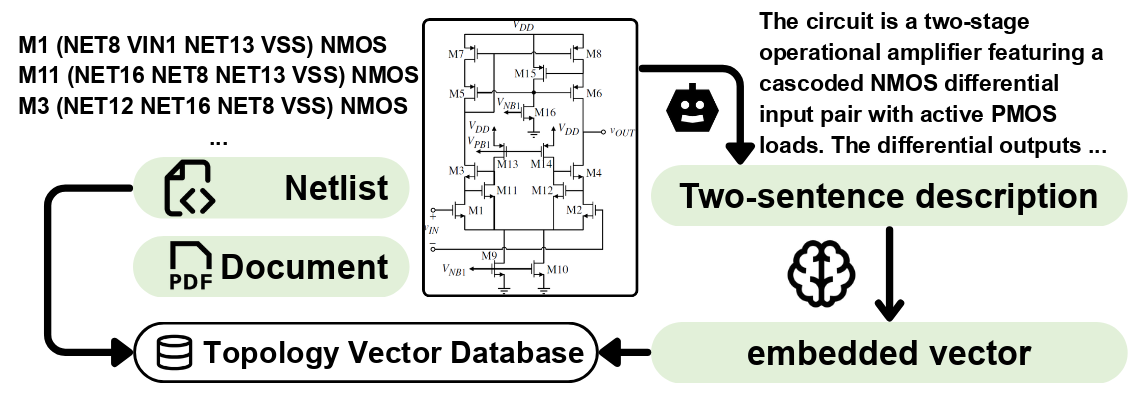
\includegraphics[width=0.4\textwidth]{image/topology.png}
    \caption{Construction workflow of the \emph{Topology Vector Database}. Each topology is converted into a two-sentence textual representation and stored as a key--value pair, where the embedded description serves as the key and the netlist as the value, enabling efficient retrieval.}
    \label{fig:topology}
\end{figure}
